\documentclass[11pt,tikz,border=3.14mm]{standalone}
\usepackage{xcolor}
\definecolor{r1}{HTML}{FF8674}
\definecolor{b1}{HTML}{17ABDD}
\definecolor{p1}{HTML}{D4B6D6}
\definecolor{g1}{HTML}{70E2CB}
\definecolor{o1}{HTML}{DFA743}

\usepackage{mathptmx}
\usepackage{BOONDOX-cal} %使用花体emf
\newcommand\EMF{\mathcal{E}} %\varepsilon}
\usepackage[outline]{contour} % glow around text
\contourlength{1.5pt}

\usepackage[european]{circuitikz}


\begin{document}
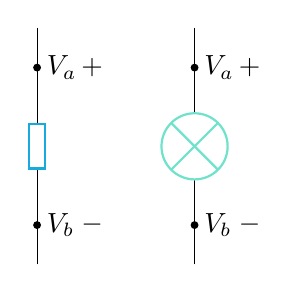
\begin{tikzpicture}
  \draw (0,0) to [R,color=b1,/tikz/circuitikz/bipoles/length=20pt](0,3);
  %\draw (2,2.5) --++ (0.6,0) to[voltmeter,color=white,name=M] ++(0,-2) --++ (-0.6,0);
  %\myvoltmeter{M}{0} % rotate
  \fill[black] (0,2.5) circle (0.05) node[right] {$V_a$};
  \fill[black] (0,0.5) circle (0.05) node[right] {$V_b$};
  \node at (0.7,2.5) {$+$};
  \node at (0.7,0.5) {$-$};

  \draw (2,0) to[lamp,color=g1] (2,3);
  %\draw (2,2.5) --++ (0.7,0) to[voltmeter,color=white,name=M] ++(0,-2) --++ (-0.7,0);
  %\myvoltmeter{M}{0} % rotate
  \fill[black] (2,2.5) circle (0.05) node[right] {$V_a$};
  \fill[black] (2,0.5) circle (0.05) node[right] {$V_b$};
  \node at (2.7,2.5) {$+$};
  \node at (2.7,0.5) {$-$};
\end{tikzpicture}

\end{document}
